\documentclass[8pt]{beamer}
\usetheme{Madrid}
\usecolortheme{default}
\usepackage{amsmath, amssymb, graphicx, array, multirow, booktabs, xcolor, tikz}
\usetikzlibrary{shapes,arrows,positioning,fit,backgrounds}

% Compact font settings
\setbeamerfont{title}{size=\Large}
\setbeamerfont{subtitle}{size=\small}
\setbeamerfont{author}{size=\scriptsize}
\setbeamerfont{date}{size=\scriptsize}
\setbeamerfont{frametitle}{size=\large}
\setbeamerfont{framesubtitle}{size=\normalsize}
\setbeamerfont{enumerate item}{size=\footnotesize}
\setbeamerfont{itemize item}{size=\footnotesize}
\setbeamerfont{block title}{size=\footnotesize}

% Compact spacing
\setlength{\itemsep}{0.08ex}
\setlength{\parskip}{0.08ex}
\setlength{\leftmargini}{0.3cm}
\setbeamersize{text margin left=3mm, text margin right=3mm}
\addtobeamertemplate{frame begin}{\vspace{-0.4cm}}{}

% Colors
\definecolor{blue}{RGB}{0,0,255}
\definecolor{red}{RGB}{255,0,0}
\definecolor{green}{RGB}{0,128,0}
\definecolor{orange}{RGB}{255,165,0}
\definecolor{purple}{RGB}{128,0,128}
\definecolor{gray}{RGB}{128,128,128}

\title{Reinforcement Learning - Part 1}
\subtitle{MAB, Monte Carlo, and TD Methods}
\author{GARP RAI Exam Preparation}
\date{}

\begin{document}

\begin{frame}
\titlepage
\end{frame}

% ============================================================
% SLIDES 1-10: INTRODUCTION
% ============================================================

\begin{frame}{TUTORIAL OVERVIEW - Part 1}
\fontsize{7}{8}\selectfont
\textbf{What You Will Learn in Part 1:}

\vspace{0.2cm}
\begin{tabular}{|p{2.5cm}|p{5.5cm}|}
\hline
\textcolor{blue}{Topic} & \textcolor{blue}{Key Concepts Covered} \\
\hline
1. RL Fundamentals & Agent, Environment, State, Action, Reward, Policy, Value Functions \\
\hline
2. Multi-Armed Bandit & Exploration vs Exploitation, $\epsilon$-Greedy, Q-Value Updates \\
\hline
3. Monte Carlo Methods & Episode-based Learning, Full Returns, Bias-Variance Trade-off \\
\hline
4. Temporal Difference & Online Learning, Bootstrapping, Q-Learning, SARSA, TD Error \\
\hline
\end{tabular}

\vspace{0.2cm}
\textbf{Key to Success:} Understand the \textcolor{blue}{"exploration vs exploitation"} trade-off!
\end{frame}

\begin{frame}{RL - What Makes It Different?}
\fontsize{6.5}{7.5}\selectfont
\textcolor{blue}{\textbf{Reinforcement Learning vs Other Paradigms}}

\begin{tabular}{|p{3.5cm}|p{5.5cm}|}
\hline
\textcolor{blue}{Paradigm} & \textcolor{blue}{Key Characteristic} \\
\hline
Supervised Learning & Learns from \textcolor{blue}{labeled data}; output = prediction/classification \\
\hline
Unsupervised Learning & Finds \textcolor{blue}{hidden patterns}; output = clusters/structures \\
\hline
Reinforcement Learning & Learns through \textcolor{blue}{trial and error}; output = policy/action \\
\hline
\end{tabular}

\textbf{Core RL Concept:}
\begin{itemize}
\item Agent \textcolor{blue}{interacts} with environment
\item Takes \textcolor{blue}{actions}
\item Receives \textcolor{blue}{rewards} (positive or negative)
\item Goal: \textcolor{blue}{Maximize cumulative future reward}
\end{itemize}

\textbf{Analogy - Dog Training:}
\begin{itemize}
\item Command $\rightarrow$ Dog takes action $\rightarrow$ Reward if correct
\item Over time, dog learns the \textcolor{blue}{policy}
\end{itemize}

\textcolor{red}{\textbf{Exam Trap:}} RL uses \textcolor{blue}{rewards}, not labels!
\end{frame}

\begin{frame}{RL - Key Terminology}
\fontsize{6.5}{7.5}\selectfont
\textcolor{blue}{\textbf{The Language of Reinforcement Learning}}

\begin{tabular}{|p{2.5cm}|p{5.5cm}|}
\hline
\textcolor{blue}{Term} & \textcolor{blue}{Definition} \\
\hline
Agent & The \textcolor{blue}{learner/decision-maker} who takes actions \\
\hline
Environment & The \textcolor{blue}{world} the agent interacts with \\
\hline
Action (a) & A \textcolor{blue}{choice} the agent can make \\
\hline
State (s) & The \textcolor{blue}{current situation} of the environment \\
\hline
Reward (R) & \textcolor{blue}{Feedback} from environment (positive or negative) \\
\hline
Policy ($\pi$) & The agent's \textcolor{blue}{strategy} - maps states to actions \\
\hline
Value Function V(s) & How \textcolor{blue}{good} it is to be in state s \\
\hline
Action-Value Q(s,a) & How \textcolor{blue}{good} it is to take action a in state s \\
\hline
\end{tabular}

\textbf{Key Insight:}
\begin{itemize}
\item Optimal policy: $\pi^*(s) = \arg\max_a Q(s,a)$
\end{itemize}

\textcolor{red}{\textbf{Exam Trap:}} Policy $\neq$ Value Function!
\end{frame}

\begin{frame}{RL - Mathematical Framework}
\fontsize{6.5}{7.5}\selectfont
\textcolor{blue}{\textbf{The Mathematics of RL}}

\textbf{Expected Future Return (G):}
\[
G_t = R_{t+1} + \gamma R_{t+2} + \gamma^2 R_{t+3} + \cdots
\]
$\gamma$ = \textcolor{blue}{discount factor} ($0 \leq \gamma \leq 1$)

\textbf{State-Value Function V(s):}
\[
V_\pi(s) = E_\pi[G_t | S_t = s]
\]

\textbf{Action-Value Function Q(s,a):}
\[
Q_\pi(s,a) = E_\pi[G_t | S_t = s, A_t = a]
\]

\textbf{Relationship:}
\[
V_\pi(s) = \sum_a \pi(a|s) Q_\pi(s,a)
\]
\[
V^*(s) = \max_a Q^*(s,a)
\]

\textcolor{red}{\textbf{Exam Trap:}} V(s) = expectation over actions; Q(s,a) = action-specific!
\end{frame}

\begin{frame}{RL - Agent-Environment Interaction}
\fontsize{6.5}{7.5}\selectfont
\textcolor{blue}{\textbf{The Agent-Environment Loop}}

\textbf{The Interaction Cycle:}
\begin{center}
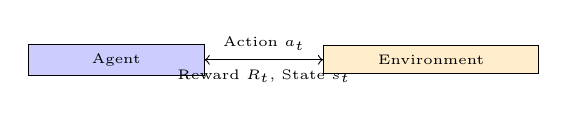
\begin{tikzpicture}[scale=0.5, every node/.style={font=\tiny}]
\node[draw, rectangle, fill=blue!20, text width=2cm, align=center] (agent) {Agent};
\node[draw, rectangle, fill=orange!20, text width=2.5cm, align=center] (env) [right of=agent, xshift=3cm] {Environment};
\draw[->] (agent) -- (env) node[midway,above] {Action $a_t$};
\draw[->] (env) -- (agent) node[midway,below] {Reward $R_t$, State $s_t$};
\end{tikzpicture}
\end{center}

\textbf{Step-by-Step:}
\begin{enumerate}
\item Agent observes \textcolor{blue}{state} $s_t$
\item Agent selects \textcolor{blue}{action} $a_t$
\item Environment returns \textcolor{blue}{reward} $R_{t+1}$ and \textcolor{blue}{next state} $s_{t+1}$
\item Agent updates its knowledge
\item Repeat
\end{enumerate}

\textbf{Formal Sequence:}
\[
s_0, a_0, R_1, s_1, a_1, R_2, s_2, a_2, R_3, ...
\]

\textcolor{red}{\textbf{Exam Trap:}} In MAB, there is only one state!
\end{frame}

\begin{frame}{RL - Famous Applications}
\fontsize{6.5}{7.5}\selectfont
\textcolor{blue}{\textbf{Real-World RL Applications}}

\textbf{AlphaGo / AlphaZero (DeepMind):}
\begin{itemize}
\item Superhuman performance in Go, Chess, Shogi
\item Played \textcolor{blue}{millions} of games against itself
\item Discovered \textcolor{blue}{novel strategies}
\end{itemize}

\textbf{Robotics:}
\begin{itemize}
\item Complex manipulation tasks
\item Self-driving cars
\item Warehouse automation
\end{itemize}

\textbf{Business:}
\begin{itemize}
\item Dynamic Pricing
\item Supply Chain Optimization
\item Algorithmic Trading
\item \textcolor{blue}{RLHF for ChatGPT} (Reinforcement Learning from Human Feedback)
\end{itemize}

\textcolor{red}{\textbf{Exam Trap:}} RLHF is key for LLM fine-tuning!
\end{frame}

\begin{frame}{RL - Challenges}
\fontsize{6.5}{7.5}\selectfont
\textcolor{blue}{\textbf{Key Challenges in RL}}

\textbf{1. Sample Efficiency:}
\begin{itemize}
\item RL requires \textcolor{red}{millions} of interactions
\item Real-world interactions can be expensive or dangerous
\end{itemize}

\textbf{2. Reward Design:}
\begin{itemize}
\item Sparse rewards make learning difficult
\item Poor reward design leads to \textcolor{red}{unintended behaviors}
\end{itemize}

\textbf{3. Computational Cost:}
\begin{itemize}
\item Deep RL requires extensive computational resources
\item Training can take days or weeks
\end{itemize}

\textbf{4. Safety and Exploration:}
\begin{itemize}
\item Exploration can be dangerous in real-world
\item Agent may take harmful actions while learning
\end{itemize}

\textbf{5. Credit Assignment:}
\begin{itemize}
\item Which actions led to the reward?
\item Delayed rewards make this difficult
\end{itemize}

\textcolor{red}{\textbf{Exam Trap:}} Sample inefficiency is RL's biggest challenge!
\end{frame}

\begin{frame}{RL - Credit Assignment Problem}
\fontsize{6.5}{7.5}\selectfont
\textcolor{blue}{\textbf{The Credit Assignment Problem}}

\textbf{What is Credit Assignment?}
\begin{itemize}
\item Determining which actions are responsible for a reward
\item In complex tasks, rewards may be \textcolor{red}{delayed}
\end{itemize}

\textbf{Example - Chess:}
\begin{itemize}
\item A move made 20 steps before checkmate contributed
\item How do we know which moves were good?
\item The reward (win/loss) comes at the end
\end{itemize}

\textbf{Solutions:}
\begin{enumerate}
\item \textcolor{blue}{Monte Carlo}: Uses complete episode returns
\item \textcolor{blue}{TD Learning}: Uses one-step or n-step returns
\item \textcolor{blue}{Eligibility Traces}: Assigns credit to recent actions
\end{enumerate}

\textbf{TD($\lambda$) Example:}
\begin{itemize}
\item $\lambda = 0$: Only immediate action gets credit
\item $\lambda = 1$: All actions get credit equally
\end{itemize}

\textcolor{red}{\textbf{Exam Trap:}} Credit assignment is the fundamental problem!
\end{frame}

\begin{frame}{RL - Exploration vs Exploitation}
\fontsize{6.5}{7.5}\selectfont
\textcolor{blue}{\textbf{The Exploration-Exploitation Dilemma}}

\textbf{Definition:}
\begin{itemize}
\item \textcolor{blue}{Exploration}: Trying new actions to gather information
\item \textcolor{blue}{Exploitation}: Using known actions to maximize reward
\end{itemize}

\textbf{Why Balance is Needed:}
\begin{itemize}
\item Pure exploitation: May miss better options (\textcolor{red}{regret})
\item Pure exploration: Never uses knowledge (\textcolor{red}{waste})
\item Optimal: Explore when uncertain, exploit when confident
\end{itemize}

\textbf{Strategies:}
\begin{enumerate}
\item \textcolor{blue}{$\epsilon$-Greedy}: Explore with probability $\epsilon$
\item \textcolor{blue}{Decaying $\epsilon$}: Explore less over time
\item \textcolor{blue}{Thompson Sampling}: Bayesian exploration
\item \textcolor{blue}{UCB}: Upper Confidence Bound
\end{enumerate}

\textbf{UCB Formula:}
\[
a_t = \arg\max_a \left( Q(a) + c \sqrt{\frac{\ln t}{N(a)}} \right)
\]

\textcolor{red}{\textbf{Exam Trap:}} UCB uses uncertainty to guide exploration!
\end{frame}

\begin{frame}{RL - Discount Factor Deep Dive}
\fontsize{6.5}{7.5}\selectfont
\textcolor{blue}{\textbf{Understanding the Discount Factor $\gamma$}}

\textbf{Why Discount?}
\begin{enumerate}
\item \textcolor{blue}{Uncertainty}: Future rewards are less certain
\item \textcolor{blue}{Time Value}: Immediate rewards are more valuable
\item \textcolor{blue}{Mathematical Convenience}: Ensures finite returns
\end{enumerate}

\textbf{Effect of $\gamma$:}
\begin{tabular}{|c|c|c|}
\hline
$\gamma$ & Behavior & Example \\
\hline
0.0 & Myopic, short-term & Immediate profit only \\
\hline
0.5 & Moderate short-term & Next few steps matter \\
\hline
0.9 & Long-term focus & Future matters significantly \\
\hline
1.0 & Infinite horizon & All future steps equal \\
\hline
\end{tabular}

\textbf{Example - Two Choices:}
\begin{itemize}
\item Choice A: $R = 100$ now
\item Choice B: $R = 10$ now, $R = 100$ later
\end{itemize}

\textbf{With $\gamma = 0.9$:}
\begin{itemize}
\item Choice A: $G = 100$
\item Choice B: $G = 10 + 0.9(100) = 100$ (Tie!)
\end{itemize}

\textbf{With $\gamma = 0.5$:}
\begin{itemize}
\item Choice A: $G = 100$
\item Choice B: $G = 10 + 0.5(100) = 60$ (Choice A better!)
\end{itemize}

\textcolor{red}{\textbf{Exam Trap:}} $\gamma$ controls time preference!
\end{frame}

% ============================================================
% SLIDES 11-25: MULTI-ARMED BANDIT
% ============================================================

\begin{frame}{MAB - Introduction}
\fontsize{6.5}{7.5}\selectfont
\textcolor{blue}{\textbf{The Multi-Armed Bandit Problem}}

\textbf{The Scenario:}
\begin{itemize}
\item Gambler faces \textcolor{blue}{multiple slot machines}
\item Each machine has \textcolor{blue}{unknown} reward distribution
\item Goal: \textcolor{blue}{Maximize total winnings}
\end{itemize}

\textbf{Key MAB Characteristics:}
\begin{enumerate}
\item \textcolor{blue}{Single state} - environment doesn't change
\item Actions don't affect future states
\item Each action gives \textcolor{blue}{immediate reward}
\item No long-term consequences
\end{enumerate}

\textbf{The Core Dilemma:}
\begin{itemize}
\item \textcolor{blue}{Exploit}: Play best machine so far
\item \textcolor{blue}{Explore}: Try other machines to find better ones
\end{itemize}

\textbf{MAB vs General RL:}
\begin{itemize}
\item MAB: Single state, no future consequences
\item General RL: Multiple states, actions affect future
\end{itemize}

\textcolor{red}{\textbf{Exam Trap:}} MAB has \textcolor{blue}{ONLY ONE STATE}!
\end{frame}

\begin{frame}{MAB - The Three Strategies}
\fontsize{6.5}{7.5}\selectfont
\textcolor{blue}{\textbf{Three Strategies for MAB}}

\textbf{Strategy 1: Greedy (Pure Exploitation)}
\begin{itemize}
\item Always choose \textcolor{blue}{highest Q-value}
\item Pros: Maximizes immediate reward
\item Cons: May miss better machine
\end{itemize}

\textbf{Strategy 2: Random (Pure Exploration)}
\begin{itemize}
\item Always choose \textcolor{blue}{random} machine
\item Pros: Gathers information about all machines
\item Cons: Never uses knowledge
\end{itemize}

\textbf{Strategy 3: $\epsilon$-Greedy (Balanced)}
\begin{itemize}
\item With probability $\epsilon$: \textcolor{blue}{Explore} (random)
\item With probability $1-\epsilon$: \textcolor{blue}{Exploit} (best)
\item \textcolor{green}{Balances} exploration and exploitation
\end{itemize}

\textbf{Decision Process:}
\begin{center}
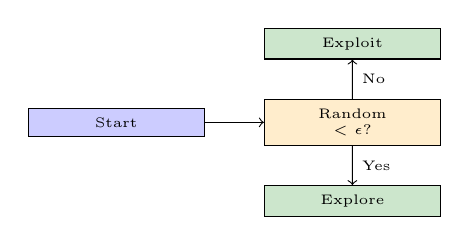
\begin{tikzpicture}[scale=0.4, every node/.style={font=\tiny}]
\node[draw, rectangle, fill=blue!20, text width=2cm, align=center] (start) {Start};
\node[draw, rectangle, fill=orange!20, text width=2cm, align=center] (rand) [right of=start, xshift=2cm] {Random\\$<$ $\epsilon$?};
\node[draw, rectangle, fill=green!20, text width=2cm, align=center] (explore) [below of=rand] {Explore};
\node[draw, rectangle, fill=green!20, text width=2cm, align=center] (exploit) [above of=rand] {Exploit};
\draw[->] (start) -- (rand);
\draw[->] (rand) -- (explore) node[midway,right] {Yes};
\draw[->] (rand) -- (exploit) node[midway,right] {No};
\end{tikzpicture}
\end{center}

\textcolor{red}{\textbf{Exam Trap:}} $\epsilon$-greedy with decay is best practical!
\end{frame}

\begin{frame}{MAB - Q-Value Calculation}
\fontsize{6.5}{7.5}\selectfont
\textcolor{blue}{\textbf{Q-Value = Average of Observed Rewards}}

\[
Q_k^n = \frac{1}{n}\sum_{j=1}^n R_j
\]

\textbf{Incremental Update:}
\[
Q_k^n = Q_k^{n-1} + \frac{1}{n}(R_n - Q_k^{n-1})
\]

\textbf{Example: Machine A played 5 times:}
\begin{itemize}
\item Rewards: [1.2, 0.8, 1.5, 0.3, 1.1]
\item Sum = 1.2 + 0.8 + 1.5 + 0.3 + 1.1 = 4.9
\item Q(A) = 4.9 / 5 = 0.98
\end{itemize}

\textbf{Step-by-Step:}
\begin{enumerate}
\item Play 1: R=1.2, Q=1.2
\item Play 2: R=0.8, Q=(1.2+0.8)/2=1.0
\item Play 3: R=1.5, Q=(1.2+0.8+1.5)/3=1.167
\item Play 4: R=0.3, Q=(1.2+0.8+1.5+0.3)/4=0.95
\item Play 5: R=1.1, Q=(1.2+0.8+1.5+0.3+1.1)/5=0.98
\end{enumerate}

\textcolor{red}{\textbf{Exam Trap:}} Q-values are \textcolor{blue}{averages}, not sums!
\end{frame}

\begin{frame}{MAB - $\epsilon$ Decay}
\fontsize{6.5}{7.5}\selectfont
\textcolor{blue}{\textbf{How $\epsilon$ Decays Over Time}}

\[
\epsilon_t = \beta^{t-1}
\]
where $\beta$ = decay factor ($0 < \beta < 1$)

\textbf{Example with $\beta = 0.85$:}

\begin{tabular}{|c|c|c|}
\hline
Trial & $\epsilon_t$ & Decision \\
\hline
1 & 1.00 & Always Explore \\
\hline
2 & 0.85 & 85\% Explore \\
\hline
5 & 0.522 & 52.2\% Explore \\
\hline
10 & 0.232 & 23.2\% Explore \\
\hline
20 & 0.046 & 4.6\% Explore \\
\hline
50 & 0.0004 & Pure Exploit \\
\hline
\end{tabular}

\textbf{Key Insight:}
\begin{itemize}
\item High $\epsilon$ early = More exploration
\item Low $\epsilon$ later = More exploitation
\item When $\epsilon$ approaches 0, agent is fully exploiting
\end{itemize}

\textbf{Linear Decay Alternative:}
\[
\epsilon_t = \epsilon_{max} - \frac{t}{T}(\epsilon_{max} - \epsilon_{min})
\]

\textcolor{red}{\textbf{Exam Trap:}} $\epsilon_t = \beta^{t-1}$, not $\beta^t$!
\end{frame}

\begin{frame}{MAB - Worked Example}
\fontsize{6.5}{7.5}\selectfont
\textcolor{blue}{\textbf{MAB - Step-by-Step Example}}

\textbf{Setup:}
\begin{itemize}
\item 3 machines: A, B, C
\item True means: $\mu_A = 0.8$, $\mu_B = 0.5$, $\mu_C = 0.7$
\item $\beta = 0.85$
\end{itemize}

\textbf{Trial 1:} $\epsilon = 1.00$, random=0.7 $\rightarrow$ Explore
\begin{itemize}
\item Choose A, Reward=1.2, Q(A)=1.2
\end{itemize}

\textbf{Trial 2:} $\epsilon = 0.85$, random=0.99 $\rightarrow$ Exploit
\begin{itemize}
\item Choose A (best), Reward=0.8, Q(A)=1.0
\end{itemize}

\textbf{Trial 3:} $\epsilon = 0.7225$, random=0.65 $\rightarrow$ Explore
\begin{itemize}
\item Choose B, Reward=1.7, Q(B)=1.7
\end{itemize}

\textbf{Trial 4:} $\epsilon = 0.614$, random=0.50 $\rightarrow$ Explore
\begin{itemize}
\item Choose C, Reward=0.6, Q(C)=0.6
\end{itemize}

\textbf{Trial 5:} $\epsilon = 0.522$, random=0.70 $\rightarrow$ Exploit
\begin{itemize}
\item Best: B (Q=1.7), Reward=0.5, Q(B)=1.1
\end{itemize}

\textbf{After 10 Trials:}
\begin{tabular}{|c|c|}
\hline
Machine & Q-Value \\
\hline
A & 0.80 \\
\hline
B & 0.50 \\
\hline
C & 0.70 \\
\hline
\end{tabular}

\textcolor{red}{\textbf{Exam Trap:}} Estimates may differ from true means due to sampling error!
\end{frame}

\begin{frame}{MAB - Greedy Strategy Risk}
\fontsize{6.5}{7.5}\selectfont
\textcolor{blue}{\textbf{The Risk of Pure Exploitation}}

\textbf{Scenario:}
\begin{itemize}
\item 3 machines after 5 plays:
\begin{itemize}
\item Q(A) = 1.5 (from 5 lucky plays)
\item Q(B) = 0.0 (never played)
\item Q(C) = 0.0 (never played)
\end{itemize}
\item True means: $\mu_A = 0.2$, $\mu_B = 2.0$, $\mu_C = 1.8$
\end{itemize}

\textbf{Greedy Strategy:}
\begin{itemize}
\item Always plays A (Q=1.5)
\item Expected reward = 0.2 per play
\item Total reward = $0.2 \times 1000 = 200$
\end{itemize}

\textbf{Optimal Strategy:}
\begin{itemize}
\item Always plays B (true mean = 2.0)
\item Total reward = $2.0 \times 1000 = 2000$
\end{itemize}

\textbf{Regret:}
\begin{itemize}
\item Regret = 2000 - 200 = 1800 (huge loss!)
\end{itemize}

\textbf{Lesson:}
\begin{itemize}
\item Greedy got \textcolor{red}{stuck} with suboptimal machine
\item \textcolor{blue}{Exploration} would have discovered better machine
\end{itemize}

\textcolor{red}{\textbf{Exam Trap:}} Greedy can be catastrophically suboptimal!
\end{frame}

\begin{frame}{MAB - Random Strategy Problem}
\fontsize{6.5}{7.5}\selectfont
\textcolor{blue}{\textbf{The Problem of Pure Exploration}}

\textbf{Scenario:}
\begin{itemize}
\item 3 machines: $\mu_A = 0.8$, $\mu_B = 0.5$, $\mu_C = 0.7$
\item 1000 plays
\end{itemize}

\textbf{Random Strategy:}
\begin{itemize}
\item Expected reward = average of all means
\item = (0.8 + 0.5 + 0.7) / 3 = 0.667
\item Total reward = $0.667 \times 1000 = 667$
\end{itemize}

\textbf{Optimal Strategy:}
\begin{itemize}
\item Always plays A (0.8)
\item Total = $0.8 \times 1000 = 800$
\end{itemize}

\textbf{Comparison:}
\begin{tabular}{|c|c|}
\hline
Strategy & Expected Reward \\
\hline
Optimal & 800 \\
\hline
$\epsilon$-greedy (0.1) & ~787 \\
\hline
Greedy (if lucky) & 800 \\
\hline
Greedy (if unlucky) & 200 \\
\hline
Random & 667 \\
\hline
\end{tabular}

\textbf{The Problem:}
\begin{itemize}
\item Random strategy \textcolor{red}{wastes} knowledge
\item After 1000 plays, knows best machine
\item But continues to play random machines!
\end{itemize}

\textcolor{red}{\textbf{Exam Trap:}} Random \textcolor{red}{never exploits} - wastes knowledge!
\end{frame}

\begin{frame}{MAB - $\epsilon$-Greedy Analysis}
\fontsize{6.5}{7.5}\selectfont
\textcolor{blue}{\textbf{$\epsilon$-Greedy - The Balanced Approach}}

\textbf{Setup:}
\begin{itemize}
\item 3 machines: $\mu_A = 0.8$, $\mu_B = 0.5$, $\mu_C = 0.7$
\item $\epsilon = 0.10$ (constant)
\item 1000 plays
\end{itemize}

\textbf{Expected Behavior:}
\begin{itemize}
\item 90\% plays: best machine (A) $\rightarrow$ reward ~0.8
\item 10\% plays: random $\rightarrow$ average ~0.667
\item Expected reward = 0.9(0.8) + 0.1(0.667) = 0.787
\item Total $\approx$ 787
\end{itemize}

\textbf{With Decay:}
\begin{itemize}
\item Early: More exploration to find best machine
\item Late: More exploitation to maximize reward
\item Often \textcolor{blue}{outperforms} constant $\epsilon$
\end{itemize}

\textbf{Why It Works:}
\begin{itemize}
\item Balances exploration and exploitation
\item Learns from experience
\item Adapts over time
\end{itemize}

\textcolor{red}{\textbf{Exam Trap:}} $\epsilon$-greedy with decay is usually better!
\end{frame}

\begin{frame}{MAB - Decay Factor Analysis}
\fontsize{6.5}{7.5}\selectfont
\textcolor{blue}{\textbf{Choosing the Decay Factor $\beta$}}

\textbf{Effect of Different $\beta$:}

\begin{tabular}{|c|c|c|c|}
\hline
Trial & $\beta=0.85$ & $\beta=0.95$ & $\beta=0.99$ \\
\hline
1 & 1.00 & 1.00 & 1.00 \\
\hline
5 & 0.522 & 0.815 & 0.961 \\
\hline
10 & 0.232 & 0.630 & 0.914 \\
\hline
20 & 0.046 & 0.377 & 0.827 \\
\hline
50 & 0.0004 & 0.077 & 0.606 \\
\hline
100 & $\approx$0 & 0.006 & 0.366 \\
\hline
200 & $\approx$0 & 0.00003 & 0.134 \\
\hline
\end{tabular}

\textbf{Interpretation:}
\begin{itemize}
\item $\beta = 0.85$: Fast decay, quick exploitation
\begin{itemize}
\item Good for simple problems
\end{itemize}
\item $\beta = 0.95$: Moderate decay, balanced
\begin{itemize}
\item Good for most practical problems
\end{itemize}
\item $\beta = 0.99$: Slow decay, long exploration
\begin{itemize}
\item Good for complex problems
\end{itemize}
\end{itemize}

\textbf{When $\epsilon$ Becomes Very Small:}
\begin{itemize}
\item $\beta=0.85$: ~57 trials
\item $\beta=0.95$: ~230 trials
\item $\beta=0.99$: ~2300 trials
\end{itemize}

\textcolor{red}{\textbf{Exam Trap:}} Smaller $\beta$ = faster decay = less exploration later!
\end{frame}

\begin{frame}{MAB - Thompson Sampling}
\fontsize{6.5}{7.5}\selectfont
\textcolor{blue}{\textbf{Thompson Sampling - A Bayesian Alternative}}

\textbf{The Concept:}
\begin{itemize}
\item Maintain \textcolor{blue}{probability distribution} for each machine
\item Sample from each distribution
\item Choose \textcolor{blue}{maximum sampled value}
\item Naturally balances exploration and exploitation
\end{itemize}

\textbf{How It Works:}
\begin{enumerate}
\item Each machine has distribution (Beta for binary, Normal for continuous)
\item Parameters update with each observation (Bayesian updating)
\item Each trial:
\begin{enumerate}
\item Sample value from each machine's distribution
\item Choose machine with highest sampled value
\item Observe reward and update distribution
\end{enumerate}
\end{enumerate}

\textbf{Example - Binary Rewards:}
\begin{itemize}
\item A: Beta(5,2) $\rightarrow$ mean=5/7=0.714
\item B: Beta(2,3) $\rightarrow$ mean=2/5=0.400
\item C: Beta(3,2) $\rightarrow$ mean=3/5=0.600
\item Sample: A=0.72, B=0.35, C=0.68 $\rightarrow$ Choose A
\end{itemize}

\textbf{Advantages:}
\begin{itemize}
\item No $\epsilon$ parameter to tune
\item Balances based on uncertainty
\item Theoretically optimal (Bayesian)
\end{itemize}

\textcolor{red}{\textbf{Exam Trap:}} Thompson Sampling is Bayesian!
\end{frame}

\begin{frame}{MAB - Regret Analysis}
\fontsize{6.5}{7.5}\selectfont
\textcolor{blue}{\textbf{Regret - Measuring Performance}}

\[
\text{Regret}(T) = T \times \mu^* - \sum_{t=1}^T \mu_{a_t}
\]

\textbf{Interpretation:}
\begin{itemize}
\item Opportunity cost of not knowing the best machine
\item Cumulative loss from suboptimal choices
\item Goal: \textcolor{blue}{Minimize regret}
\end{itemize}

\textbf{Example:}
\begin{itemize}
\item True means: $\mu_A = 0.8$, $\mu_B = 0.5$, $\mu_C = 0.7$
\item $\mu^* = 0.8$ (Machine A)
\item If agent plays Machine B 100 times:
\begin{itemize}
\item Regret per play = 0.8 - 0.5 = 0.3
\item Total regret = 0.3 $\times$ 100 = 30
\end{itemize}
\end{itemize}

\textbf{Expected Regret (T=1000):}
\begin{tabular}{|c|c|}
\hline
Strategy & Expected Regret \\
\hline
Optimal & 0 \\
\hline
$\epsilon$-greedy (0.1) & ~13 \\
\hline
Greedy (unlucky) & ~600 \\
\hline
Random & ~133 \\
\hline
\end{tabular}

\textbf{Key Insight:}
\begin{itemize}
\item Good algorithms achieve \textcolor{blue}{sublinear regret}
\item $\epsilon$-greedy with decay achieves $O(\log T)$ regret
\end{itemize}

\textcolor{red}{\textbf{Exam Trap:}} Regret is cumulative loss - minimize it!
\end{frame}

\begin{frame}{MAB - A/B Testing Application}
\fontsize{6.5}{7.5}\selectfont
\textcolor{blue}{\textbf{A/B Testing as a Multi-Armed Bandit}}

\textbf{Traditional A/B Testing:}
\begin{itemize}
\item Split traffic 50/50 between options
\item Test for statistical significance
\item Then implement the winner
\item Problem: \textcolor{red}{Wastes traffic} on inferior options
\end{itemize}

\textbf{MAB Approach:}
\begin{itemize}
\item Each variant = \textcolor{blue}{slot machine}
\item Use $\epsilon$-greedy or Thompson Sampling
\item Dynamically allocate more traffic to better variants
\end{itemize}

\textbf{Example - Ad Click-Through Rates:}
\begin{itemize}
\item Variant A: 5\% CTR (true)
\item Variant B: 3\% CTR (true)
\item Variant C: 4\% CTR (true)
\end{itemize}

\textbf{Traditional (100,000 impressions):}
\begin{itemize}
\item Each variant gets 33,333 impressions
\item Expected clicks = 0.05(33,333)+0.03(33,333)+0.04(33,333) = 4,000
\end{itemize}

\textbf{MAB Approach:}
\begin{itemize}
\item Early: Explore all variants
\item Later: ~90\% to best (A)
\item Expected clicks $\approx$ 4,850
\item \textcolor{green}{21\% more clicks!}
\end{itemize}

\textcolor{red}{\textbf{Exam Trap:}} MAB significantly outperforms A/B testing!
\end{frame}

\begin{frame}{MAB - Summary}
\fontsize{6.5}{7.5}\selectfont
\textcolor{blue}{\textbf{MAB - Key Takeaways}}

\textbf{Key Concepts:}
\begin{enumerate}
\item \textcolor{blue}{MAB Characteristics:}
\begin{itemize}
\item Single state, immediate rewards, no future consequences
\end{itemize}

\item \textcolor{blue}{Three Strategies:}
\begin{itemize}
\item Greedy = Pure exploitation
\item Random = Pure exploration
\item $\epsilon$-Greedy = Balanced (best)
\end{itemize}

\item \textcolor{blue}{Q-Value:}
\[
Q_k^n = \frac{1}{n}\sum R_j
\]

\item \textcolor{blue}{$\epsilon$ Decay:}
\[
\epsilon_t = \beta^{t-1}
\]

\item \textcolor{blue}{Regret:}
\begin{itemize}
\item Loss from not knowing the optimal action
\end{itemize}

\item \textcolor{blue}{Thompson Sampling:}
\begin{itemize}
\item Bayesian approach, no $\epsilon$ parameter
\end{itemize}
\end{enumerate}

\textcolor{red}{\textbf{Exam Success:}} MAB is the foundation - master it!
\end{frame}

% ============================================================
% SLIDES 26-40: MONTE CARLO METHODS
% ============================================================

\begin{frame}{Monte Carlo - Introduction}
\fontsize{6.5}{7.5}\selectfont
\textcolor{blue}{\textbf{Monte Carlo - Learning from Complete Episodes}}

\textbf{What is Monte Carlo RL?}
\begin{itemize}
\item Learns from \textcolor{blue}{complete episodes}
\item Episode = full sequence from start to terminal state
\item Example: Complete game of chess
\end{itemize}

\textbf{Key Characteristics:}
\begin{itemize}
\item \textcolor{blue}{Wait until episode ends} to update
\item Uses \textcolor{blue}{actual returns} ($G_t$)
\item \textcolor{green}{Unbiased} - learns from real experience
\end{itemize}

\textbf{MC vs MAB:}
\begin{itemize}
\item MAB: Each trial independent, one-step
\item MC: Multiple steps, actions affect future states
\end{itemize}

\textbf{When to Use MC:}
\begin{itemize}
\item Tasks with \textcolor{blue}{defined terminal states} (episodic)
\item When you want \textcolor{blue}{unbiased} estimates
\item When episodes are not too long
\end{itemize}

\textbf{Update Formula:}
\[
Q(s,a) \leftarrow Q(s,a) + \alpha(G_t - Q(s,a))
\]

\textcolor{red}{\textbf{Exam Trap:}} MC requires \textcolor{blue}{complete episodes}!
\end{frame}

\begin{frame}{Monte Carlo - Episode Definition}
\fontsize{6.5}{7.5}\selectfont
\textcolor{blue}{\textbf{What is an Episode?}}

\textbf{Definition:}
\begin{itemize}
\item Complete trajectory from start to terminal state
\item Sequence: $S_0, A_0, R_1, S_1, A_1, ..., S_T$
\item Terminal state $S_T$ ends the episode
\end{itemize}

\textbf{Examples:}
\begin{enumerate}
\item \textcolor{blue}{Nim}: Start $\rightarrow$ coin removal $\rightarrow$ last coin wins
\item \textcolor{blue}{Chess}: Opening $\rightarrow$ moves $\rightarrow$ Checkmate
\item \textcolor{blue}{Board Game}: Start $\rightarrow$ moves $\rightarrow$ Win/Lose
\end{enumerate}

\textbf{Return Calculation:}
\[
G_t = R_{t+1} + \gamma R_{t+2} + \cdots + \gamma^{T-t-1}R_T
\]

\textbf{Nim Example:}
\begin{itemize}
\item Episode length: 3 steps (if Player 1 wins)
\item Step 1: Pick 3 coins (S=6 $\rightarrow$ S=3)
\item Step 2: Opponent picks 2 coins (S=3 $\rightarrow$ S=1)
\item Step 3: Player 1 picks 1 coin (S=1 $\rightarrow$ S=0, Win!)
\end{itemize}

\textbf{Update Only at Episode End:}
\begin{itemize}
\item No updates within episode
\item All state-action pairs updated at end
\end{itemize}

\textcolor{red}{\textbf{Exam Trap:}} MC updates \textcolor{blue}{only at episode end}!
\end{frame}

\begin{frame}{Monte Carlo - Return Calculation}
\fontsize{6.5}{7.5}\selectfont
\textcolor{blue}{\textbf{Calculating Returns in MC}}

\[
G_t = \sum_{k=0}^{T-t-1} \gamma^k R_{t+k+1}
\]

\textbf{Example - Nim with $\gamma = 1$:}
\begin{itemize}
\item Episode: S=6 $\rightarrow$ S=3 $\rightarrow$ S=1 $\rightarrow$ S=0 (Win)
\item Rewards: $R_1=0, R_2=0, R_3=1$
\item For step 1 (t=0): $G_0 = 0 + 0 + 1 = 1$
\item For step 2 (t=1): $G_1 = 0 + 1 = 1$
\item For step 3 (t=2): $G_2 = 1$
\end{itemize}

\textbf{Example - Nim with $\gamma = 0.9$:}
\begin{itemize}
\item $G_0 = R_1 + 0.9R_2 + 0.9^2R_3 = 0 + 0 + 0.81 = 0.81$
\item $G_1 = R_2 + 0.9R_3 = 0 + 0.9 = 0.9$
\item $G_2 = R_3 = 1$
\end{itemize}

\textbf{Why Discount?}
\begin{itemize}
\item Future rewards are less certain
\item Discounting gives more weight to immediate rewards
\item $\gamma$ close to 0: Short-term focus
\item $\gamma$ close to 1: Long-term focus
\end{itemize}

\textcolor{red}{\textbf{Exam Trap:}} MC uses actual return $G_t$!
\end{frame}

\begin{frame}{Monte Carlo - First-Visit vs Every-Visit}
\fontsize{6.5}{7.5}\selectfont
\textcolor{blue}{\textbf{First-Visit vs Every-Visit MC}}

\textbf{The Distinction:}
\begin{itemize}
\item In an episode, same state-action pair $(s,a)$ may be visited multiple times
\item Two ways to handle this:
\end{itemize}

\textbf{First-Visit MC:}
\begin{itemize}
\item Track which $(s,a)$ have been seen
\item Only update Q(s,a) the \textcolor{blue}{first time} it occurs
\item Uses return from that first occurrence
\item \textcolor{green}{Unbiased} estimate of Q(s,a)
\end{itemize}

\textbf{Every-Visit MC:}
\begin{itemize}
\item Update Q(s,a) \textcolor{blue}{every time} it occurs
\item Uses return from each occurrence
\item \textcolor{orange}{Slightly biased} but often lower variance
\end{itemize}

\textbf{Example:}
\begin{itemize}
\item Episode: (S1,A1), (S2,A2), (S1,A1), (S3,A3), Terminal
\item First-visit: Update (S1,A1) once (using first occurrence)
\item Every-visit: Update (S1,A1) twice (both occurrences)
\end{itemize}

\textbf{When to Use:}
\begin{itemize}
\item First-visit: Theoretical purity, unbiased estimates
\item Every-visit: More sample-efficient, practical use
\end{itemize}

\textcolor{red}{\textbf{Exam Trap:}} First-visit = unbiased; Every-visit = lower variance!
\end{frame}

\begin{frame}{Monte Carlo - NIM Example Step 1}
\fontsize{6.5}{7.5}\selectfont
\textcolor{blue}{\textbf{MC NIM - First Episode}}

\textbf{Setup:}
\begin{itemize}
\item 6 coins, remove 1, 2, or 3
\item $\alpha = 0.05$, $\gamma = 1$
\item Opponent plays randomly (not optimally)
\end{itemize}

\textbf{Episode 1:}
\begin{enumerate}
\item S=6, A=3 $\rightarrow$ S'=3 (opponent picks 2)
\item S=1, A=1 $\rightarrow$ S'=0 (Player 1 wins!)
\item Return: $G = 1$ (win)
\end{enumerate}

\textbf{MC Updates (Episode End):}
\begin{itemize}
\item For (6,3): $Q(6,3) = 0 + 0.05(1 - 0) = 0.05$
\item For (1,1): $Q(1,1) = 0 + 0.05(1 - 0) = 0.05$
\end{itemize}

\textbf{After Episode 1:}
\begin{tabular}{|c|c|c|c|c|c|c|}
\hline
Action & S=1 & S=2 & S=3 & S=4 & S=5 & S=6 \\
\hline
Pick 1 & 0.05 & 0 & 0 & 0 & 0 & 0 \\
\hline
Pick 2 & 0 & 0 & 0 & 0 & 0 & 0 \\
\hline
Pick 3 & 0 & 0 & 0 & 0 & 0 & 0.05 \\
\hline
\end{tabular}

\textcolor{red}{\textbf{Exam Trap:}} MC updates all pairs in episode with same G!
\end{frame}

\begin{frame}{Monte Carlo - NIM Example Step 2}
\fontsize{6.5}{7.5}\selectfont
\textcolor{blue}{\textbf{MC NIM - Second Episode}}

\textbf{Episode 2:}
\begin{enumerate}
\item S=6, A=1 $\rightarrow$ S'=5 (opponent picks 1)
\item S=4, A=3 $\rightarrow$ S'=1 (opponent picks 1)
\item S=0 (Player 1 loses!)
\item Return: $G = -1$ (loss)
\end{enumerate}

\textbf{MC Updates (Episode End):}
\begin{itemize}
\item For (6,1): $Q(6,1) = 0 + 0.05(-1 - 0) = -0.05$
\item For (4,3): $Q(4,3) = 0 + 0.05(-1 - 0) = -0.05$
\end{itemize}

\textbf{After Episode 2:}
\begin{tabular}{|c|c|c|c|c|c|c|}
\hline
Action & S=1 & S=2 & S=3 & S=4 & S=5 & S=6 \\
\hline
Pick 1 & 0.05 & 0 & 0 & 0 & 0 & -0.05 \\
\hline
Pick 2 & 0 & 0 & 0 & 0 & 0 & 0 \\
\hline
Pick 3 & 0 & 0 & 0 & -0.05 & 0 & 0.05 \\
\hline
\end{tabular}

\textcolor{red}{\textbf{Exam Trap:}} Negative G updates Q-values downward!
\end{frame}

\begin{frame}{Monte Carlo - NIM Example Step 3}
\fontsize{6.5}{7.5}\selectfont
\textcolor{blue}{\textbf{MC NIM - Third Episode}}

\textbf{Episode 3:}
\begin{enumerate}
\item S=6, A=3 $\rightarrow$ S'=3 (opponent picks 2)
\item S=1, A=1 $\rightarrow$ S'=0 (Player 1 wins!)
\item Return: $G = 1$
\end{enumerate}

\textbf{MC Updates:}
\begin{itemize}
\item Q(6,3) = 0.05 + 0.05(1 - 0.05) = 0.0975
\item Q(1,1) = 0.05 + 0.05(1 - 0.05) = 0.0975
\end{itemize}

\textbf{After Episode 3:}
\begin{tabular}{|c|c|c|c|c|c|c|}
\hline
Action & S=1 & S=2 & S=3 & S=4 & S=5 & S=6 \\
\hline
Pick 1 & 0.0975 & 0 & 0 & 0 & 0 & -0.05 \\
\hline
Pick 2 & 0 & 0 & 0 & 0 & 0 & 0 \\
\hline
Pick 3 & 0 & 0 & 0 & -0.05 & 0 & 0.0975 \\
\hline
\end{tabular}

\textcolor{red}{\textbf{Exam Trap:}} Q-values gradually move toward true values!
\end{frame}

\begin{frame}{Monte Carlo - NIM Final Results}
\fontsize{6.5}{7.5}\selectfont
\textcolor{blue}{\textbf{MC NIM - After 1,000,000 Episodes}}

\textbf{Final Q-Table:}
\begin{tabular}{|c|c|c|c|c|c|c|}
\hline
Action & S=1 & S=2 & S=3 & S=4 & S=5 & S=6 \\
\hline
Pick 1 & 1 & -1 & -0.071 & 0.380 & 0 & 0.774 \\
\hline
Pick 2 & 0 & 1 & -1 & -0.110 & 0 & 1 \\
\hline
Pick 3 & 0 & 0 & 1 & -0.858 & 0 & 0.020 \\
\hline
\end{tabular}

\textbf{Optimal Strategy:}
\begin{itemize}
\item S=6: Pick 2 (Q=1)
\item S=4: Pick 1 (Q=0.380)
\item S=3: Pick 3 (Q=1)
\item S=2: Pick 2 (Q=1)
\item S=1: Pick 1 (Q=1)
\end{itemize}

\textbf{Interpretation:}
\begin{itemize}
\item Q=1 = winning action
\item Q=-1 = losing action
\item Optimal strategy ensures win
\end{itemize}

\textcolor{red}{\textbf{Exam Trap:}} Q=1 = winning action; Q=-1 = losing action!
\end{frame}

\begin{frame}{Monte Carlo - Advantages and Disadvantages}
\fontsize{6.5}{7.5}\selectfont
\textcolor{blue}{\textbf{MC - Pros and Cons}}

\textbf{Advantages:}
\begin{enumerate}
\item \textcolor{green}{Unbiased estimates} - uses actual returns
\item \textcolor{green}{Simple to understand and implement}
\item \textcolor{green}{Works well with long episodes}
\item \textcolor{green}{No bootstrapping} - no risk of propagating errors
\end{enumerate}

\textbf{Disadvantages:}
\begin{enumerate}
\item \textcolor{red}{High variance} - returns can fluctuate significantly
\item \textcolor{red}{Requires complete episodes} - cannot handle continuous tasks
\item \textcolor{red}{Slow learning} - must wait until episode end
\item \textcolor{red}{Inefficient for long episodes} - updates are infrequent
\end{enumerate}

\textbf{When to Use MC:}
\begin{itemize}
\item Tasks with clear terminal states (episodic)
\item When you can run many episodes
\item When you want unbiased value estimates
\end{itemize}

\textbf{Comparison:}
\begin{tabular}{|c|c|}
\hline
MC & TD \\
\hline
Unbiased & Biased \\
\hline
High variance & Low variance \\
\hline
Episode-end & Step-by-step \\
\hline
Episodic only & Episodic + Continuous \\
\hline
\end{tabular}

\textcolor{red}{\textbf{Exam Trap:}} MC = unbiased but high variance!
\end{frame}

\begin{frame}{Monte Carlo - Summary}
\fontsize{6.5}{7.5}\selectfont
\textcolor{blue}{\textbf{Monte Carlo - Key Takeaways}}

\textbf{Key Concepts:}
\begin{enumerate}
\item \textcolor{blue}{Definition:}
\begin{itemize}
\item Learns from complete episodes
\item Updates only at episode end
\item Uses actual returns ($G_t$)
\end{itemize}

\item \textcolor{blue}{Update Formula:}
\[
Q(s,a) \leftarrow Q(s,a) + \alpha(G_t - Q(s,a))
\]

\item \textcolor{blue}{Return Calculation:}
\[
G_t = R_{t+1} + \gamma R_{t+2} + \cdots
\]

\item \textcolor{blue}{First-Visit vs Every-Visit:}
\begin{itemize}
\item First-visit: unbiased
\item Every-visit: lower variance
\end{itemize}

\item \textcolor{blue}{Requirements:}
\begin{itemize}
\item \textcolor{red}{Must have} terminal states (episodic tasks)
\item Cannot handle continuous tasks
\end{itemize}

\item \textcolor{blue}{Trade-off:}
\begin{itemize}
\item \textcolor{green}{Unbiased} but \textcolor{red}{high variance}
\end{itemize}
\end{enumerate}

\textcolor{red}{\textbf{Exam Success:}} MC = episodic tasks only!
\end{frame}

% ============================================================
% SLIDES 41-50: TEMPORAL DIFFERENCE (PART 1)
% ============================================================

\begin{frame}{TD - Introduction}
\fontsize{6.5}{7.5}\selectfont
\textcolor{blue}{\textbf{Temporal Difference - Learning Step by Step}}

\textbf{What is TD Learning?}
\begin{itemize}
\item Learns from \textcolor{blue}{incomplete episodes}
\item Updates \textcolor{blue}{after each step} (online learning)
\item Uses \textcolor{blue}{bootstrapping} - estimates of future values
\end{itemize}

\textbf{Key Characteristic:}
\begin{itemize}
\item \textcolor{blue}{Doesn't wait} for episode end
\item Updates using $R_{t+1} + \gamma V(s')$
\item \textcolor{orange}{Biased} but \textcolor{green}{lower variance}
\end{itemize}

\textbf{TD vs MC:}
\begin{tabular}{|c|c|}
\hline
MC & TD \\
\hline
Episode-end updates & Step-by-step updates \\
\hline
Uses $G_t$ (actual return) & Uses $R_{t+1} + \gamma V(s')$ (estimate) \\
\hline
Unbiased & Biased (bootstrapping) \\
\hline
High variance & Low variance \\
\hline
Episodic only & Episodic + Continuous \\
\hline
\end{tabular}

\textbf{TD Update Formula:}
\[
V(s) \leftarrow V(s) + \alpha(R_{t+1} + \gamma V(s') - V(s))
\]

\textbf{TD Error:}
\[
\delta = R_{t+1} + \gamma V(s') - V(s)
\]
= the \textcolor{blue}{"surprise"}

\textcolor{red}{\textbf{Exam Trap:}} TD uses bootstrapping!
\end{frame}

\begin{frame}{TD - Bootstrapping Explained}
\fontsize{6.5}{7.5}\selectfont
\textcolor{blue}{\textbf{Bootstrapping - The Core of TD}}

\textbf{What is Bootstrapping?}
\begin{itemize}
\item Using a \textcolor{blue}{current estimate} to update another estimate
\item "Pulling yourself up by your own bootstraps"
\item Instead of waiting for final outcome, use current best guess
\end{itemize}

\textbf{MC vs TD Bootstrapping:}
\begin{itemize}
\item \textcolor{blue}{MC}: No bootstrapping - uses actual returns
\item \textcolor{blue}{TD}: Bootstrapping - uses estimates of future values
\end{itemize}

\textbf{Example - Nim:}
\begin{itemize}
\item S=6, take action that leads to S'=1
\item MC: Wait until episode end to know $G$
\item TD: Use $V(1)$ (current estimate) + immediate reward
\end{itemize}

\textbf{TD Target:}
\[
R_{t+1} + \gamma V(s')
\]
\begin{itemize}
\item Better guess than $V(s)$ alone
\item Uses immediate reward + estimate of future
\end{itemize}

\textbf{Why Bootstrapping Works:}
\begin{itemize}
\item Updates can be made immediately
\item Doesn't require complete episodes
\item Often converges faster than MC
\end{itemize}

\textbf{TD Error:}
\[
\delta = R_{t+1} + \gamma V(s') - V(s)
\]
\begin{itemize}
\item Positive: State better than thought
\item Negative: State worse than thought
\item Zero: Matches current estimate
\end{itemize}

\textcolor{red}{\textbf{Exam Trap:}} Bootstrapping introduces bias but reduces variance!
\end{frame}

\begin{frame}{TD - Q-Learning}
\fontsize{6.5}{7.5}\selectfont
\textcolor{blue}{\textbf{Q-Learning - The Most Popular TD Algorithm}}

\textbf{Update Formula:}
\[
Q(s,a) \leftarrow Q(s,a) + \alpha(R_{t+1} + \gamma \max_{a'} Q(s',a') - Q(s,a))
\]

\textbf{Key Features:}
\begin{enumerate}
\item \textcolor{blue}{Off-policy}: Learns optimal policy regardless of behavior
\item \textcolor{blue}{Model-free}: No environment model needed
\item \textcolor{blue}{TD method}: Uses bootstrapping
\end{enumerate}

\textbf{Why Off-Policy?}
\begin{itemize}
\item Uses $\max_{a'} Q(s',a')$ (best possible action)
\item Doesn't matter which action was actually taken
\item Learns about \textcolor{blue}{optimal policy}
\end{itemize}

\textbf{Algorithm Steps:}
\begin{enumerate}
\item Initialize Q(s,a) arbitrarily
\item For each episode:
\begin{enumerate}
\item Initialize state s
\item For each step:
\begin{enumerate}
\item Choose a from s using $\epsilon$-greedy
\item Take action a, observe R and s'
\item Update Q(s,a) using TD target
\item s $\leftarrow$ s'
\end{enumerate}
\end{enumerate}
\end{enumerate}

\textbf{Convergence Properties:}
\begin{itemize}
\item Converges to optimal Q* with probability 1
\item Requires all state-action pairs visited infinitely often
\end{itemize}

\textcolor{red}{\textbf{Exam Trap:}} Q-learning is off-policy!
\end{frame}

\begin{frame}{TD - SARSA}
\fontsize{6.5}{7.5}\selectfont
\textcolor{blue}{\textbf{SARSA - On-Policy TD Learning}}

\textbf{Update Formula:}
\[
Q(s,a) \leftarrow Q(s,a) + \alpha(R_{t+1} + \gamma Q(s',a') - Q(s,a))
\]
where $a'$ is the \textcolor{blue}{actual action} taken in $s'$

\textbf{Key Features:}
\begin{enumerate}
\item \textcolor{blue}{On-policy}: Learns the policy being followed
\item \textcolor{blue}{Model-free}: No environment model needed
\item \textcolor{blue}{TD method}: Uses bootstrapping
\end{enumerate}

\textbf{Why On-Policy?}
\begin{itemize}
\item Uses $Q(s',a')$ where $a'$ is actual next action
\item Learns about \textcolor{blue}{current policy}, not optimal
\item Policy and learning are linked
\end{itemize}

\textbf{SARSA vs Q-Learning:}
\begin{tabular}{|c|c|}
\hline
Q-Learning & SARSA \\
\hline
Off-policy & On-policy \\
\hline
Uses $\max_{a'} Q(s',a')$ & Uses $Q(s',a')$ (actual) \\
\hline
More aggressive & More conservative \\
\hline
Learns optimal & Learns current \\
\hline
\end{tabular}

\textbf{Algorithm Steps:}
\begin{enumerate}
\item Initialize Q(s,a)
\item For each episode:
\begin{enumerate}
\item Choose a from s using policy
\item For each step:
\begin{enumerate}
\item Take action, observe R, s'
\item Choose a' from s' using policy
\item Update Q(s,a) using Q(s',a')
\item s $\leftarrow$ s', a $\leftarrow$ a'
\end{enumerate}
\end{enumerate}
\end{enumerate}

\textcolor{red}{\textbf{Exam Trap:}} SARSA is on-policy; Q-learning is off-policy!
\end{frame}

\begin{frame}{TD - Q-Learning vs SARSA Comparison}
\fontsize{6.5}{7.5}\selectfont
\textcolor{blue}{\textbf{Q-Learning vs SARSA - Detailed Comparison}}

\textbf{Key Difference:}
\begin{itemize}
\item Q-learning: $R + \gamma \max_{a'} Q(s',a')$
\item SARSA: $R + \gamma Q(s',a')$
\end{itemize}

\textbf{Behavioral Differences:}
\begin{tabular}{|c|c|}
\hline
Q-Learning & SARSA \\
\hline
Best possible next action & Actual next action \\
\hline
More aggressive & More conservative \\
\hline
Learns risky policies & Learns safe policies \\
\hline
May choose danger if avoided optimally & May avoid danger under current policy \\
\hline
\end{tabular}

\textbf{Example - Cliff Walking:}
\begin{itemize}
\item Agent must walk along cliff to reach goal
\item Falling off cliff = large negative reward
\end{itemize}

\textbf{Q-Learning:}
\begin{itemize}
\item Learns optimal path (right next to cliff)
\item Risky if agent sometimes makes mistakes
\end{itemize}

\textbf{SARSA:}
\begin{itemize}
\item Learns safer path (further from cliff)
\item Accounts for suboptimal actions
\end{itemize}

\textbf{Which to Use?}
\begin{itemize}
\item Q-learning: Want optimal policy, can explore safely
\item SARSA: Safety important, exploration is risky
\end{itemize}

\textcolor{red}{\textbf{Exam Trap:}} Q-learning = aggressive; SARSA = conservative!
\end{frame}

\begin{frame}{TD - NIM Example Step 1}
\fontsize{6.5}{7.5}\selectfont
\textcolor{blue}{\textbf{TD NIM - First Episode}}

\textbf{Setup:}
\begin{itemize}
\item 6 coins, remove 1, 2, or 3
\item $\alpha = 0.05$, $\gamma = 1$
\item Opponent plays randomly
\end{itemize}

\textbf{Episode 1:}
\begin{enumerate}
\item S=6, A=3 $\rightarrow$ S'=3, R=0
\item S=1, A=1 $\rightarrow$ S'=0, R=1 (Win!)
\end{enumerate}

\textbf{TD Updates (Step by Step):}
\begin{itemize}
\item \textbf{Step 1:} S=6, A=3, S'=3, R=0
\begin{itemize}
\item V(3) = 0 (current estimate)
\item TD target = $0 + 1(0) = 0$
\item Q(6,3) = $0 + 0.05(0 - 0) = 0$
\end{itemize}
\item \textbf{Step 2:} S=1, A=1, S'=0, R=1
\begin{itemize}
\item V(0) = 0 (terminal state)
\item TD target = $1 + 1(0) = 1$
\item Q(1,1) = $0 + 0.05(1 - 0) = 0.05$
\end{itemize}
\item Update V(1): V(1) = max Q(1,a) = 0.05
\end{itemize}

\textbf{After Episode 1:}
\begin{tabular}{|c|c|c|c|c|c|c|}
\hline
Action & S=1 & S=2 & S=3 & S=4 & S=5 & S=6 \\
\hline
Pick 1 & 0.05 & 0 & 0 & 0 & 0 & 0 \\
\hline
Pick 2 & 0 & 0 & 0 & 0 & 0 & 0 \\
\hline
Pick 3 & 0 & 0 & 0 & 0 & 0 & 0 \\
\hline
\end{tabular}

\textcolor{red}{\textbf{Exam Trap:}} TD updates within episode using V(s')!
\end{frame}

\begin{frame}{TD - NIM Example Step 2}
\fontsize{6.5}{7.5}\selectfont
\textcolor{blue}{\textbf{TD NIM - Second Episode}}

\textbf{Episode 2:}
\begin{enumerate}
\item S=6, A=1 $\rightarrow$ S'=5, R=0
\item S=4, A=3 $\rightarrow$ S'=1, R=0
\item S=0 (Player 1 loses!)
\end{enumerate}

\textbf{TD Updates:}
\begin{itemize}
\item \textbf{Step 1:} S=6, A=1, S'=5, R=0
\begin{itemize}
\item V(5) = 0
\item TD target = $0 + 1(0) = 0$
\item Q(6,1) = 0 + 0.05(0 - 0) = 0
\end{itemize}
\item \textbf{Step 2:} S=4, A=3, S'=1, R=0
\begin{itemize}
\item V(1) = 0.05 (from Episode 1)
\item TD target = $0 + 1(0.05) = 0.05$
\item Q(4,3) = 0 + 0.05(0.05 - 0) = 0.0025
\end{itemize}
\end{itemize}

\textbf{After Episode 2:}
\begin{tabular}{|c|c|c|c|c|c|c|}
\hline
Action & S=1 & S=2 & S=3 & S=4 & S=5 & S=6 \\
\hline
Pick 1 & 0.05 & 0 & 0 & 0 & 0 & 0 \\
\hline
Pick 2 & 0 & 0 & 0 & 0 & 0 & 0 \\
\hline
Pick 3 & 0 & 0 & 0 & 0.0025 & 0 & 0 \\
\hline
\end{tabular}
V(1) = 0.05, V(4) = 0.0025

\textcolor{red}{\textbf{Exam Trap:}} TD uses V(1) from previous episode!
\end{frame}

\begin{frame}{TD - NIM Example Step 3}
\fontsize{6.5}{7.5}\selectfont
\textcolor{blue}{\textbf{TD NIM - Third Episode}}

\textbf{Episode 3:}
\begin{enumerate}
\item S=6, A=3 $\rightarrow$ S'=1, R=0
\item S=1, A=1 $\rightarrow$ S'=0, R=1 (Win!)
\end{enumerate}

\textbf{TD Updates:}
\begin{itemize}
\item \textbf{Step 1:} S=6, A=3, S'=1, R=0
\begin{itemize}
\item V(1) = 0.05 (from Episode 1)
\item TD target = $0 + 1(0.05) = 0.05$
\item Q(6,3) = 0 + 0.05(0.05 - 0) = 0.0025
\end{itemize}
\item \textbf{Step 2:} S=1, A=1, S'=0, R=1
\begin{itemize}
\item TD target = $1 + 1(0) = 1$
\item Q(1,1) = 0.05 + 0.05(1 - 0.05) = 0.0975
\end{itemize}
\end{itemize}

\textbf{After Episode 3:}
\begin{tabular}{|c|c|c|c|c|c|c|}
\hline
Action & S=1 & S=2 & S=3 & S=4 & S=5 & S=6 \\
\hline
Pick 1 & 0.0975 & 0 & 0 & 0 & 0 & 0 \\
\hline
Pick 2 & 0 & 0 & 0 & 0 & 0 & 0 \\
\hline
Pick 3 & 0 & 0 & 0 & 0.0025 & 0 & 0.0025 \\
\hline
\end{tabular}

\textcolor{red}{\textbf{Exam Trap:}} TD values propagate backward through episode!
\end{frame}

\begin{frame}{TD - NIM Final Results}
\fontsize{6.5}{7.5}\selectfont
\textcolor{blue}{\textbf{TD NIM - After 1,000,000 Episodes}}

\textbf{Final Q-Table:}
\begin{tabular}{|c|c|c|c|c|c|c|}
\hline
Action & S=1 & S=2 & S=3 & S=4 & S=5 & S=6 \\
\hline
Pick 1 & 1 & -1 & -0.105 & 0.383 & 0 & 0.845 \\
\hline
Pick 2 & 0 & 1 & -1 & 0.058 & 0 & 1 \\
\hline
Pick 3 & 0 & 0 & 1 & -0.842 & 0 & 0.011 \\
\hline
\end{tabular}

\textbf{Optimal Strategy:}
\begin{itemize}
\item S=6: Pick 2
\item S=4: Pick 1
\item S=3: Pick 3
\item S=2: Pick 2
\item S=1: Pick 1
\end{itemize}

\textbf{Key Insight:}
\begin{itemize}
\item Both MC and TD converge to \textcolor{blue}{same optimal strategy}
\item TD learns faster than MC
\end{itemize}

\textcolor{red}{\textbf{Exam Trap:}} Both MC and TD converge to optimal policy!
\end{frame}

\begin{frame}{TD - Advantages and Disadvantages}
\fontsize{6.5}{7.5}\selectfont
\textcolor{blue}{\textbf{TD - Pros and Cons}}

\textbf{Advantages:}
\begin{enumerate}
\item \textcolor{green}{Can learn online} - updates after each step
\item \textcolor{green}{Works for continuous tasks}
\item \textcolor{green}{Lower variance} than MC
\item \textcolor{green}{More sample efficient}
\item \textcolor{green}{Often converges faster}
\end{enumerate}

\textbf{Disadvantages:}
\begin{enumerate}
\item \textcolor{red}{Biased} - uses estimates
\item \textcolor{red}{May propagate errors}
\item \textcolor{red}{Requires careful tuning}
\item \textcolor{red}{Can be unstable}
\end{enumerate}

\textbf{When to Use TD:}
\begin{itemize}
\item Continuous (non-episodic) tasks
\item When you need online learning
\item When episodes are very long
\item When you want faster learning
\end{itemize}

\textbf{Comparison:}
\begin{tabular}{|c|c|}
\hline
MC & TD \\
\hline
Unbiased & Biased \\
\hline
High variance & Low variance \\
\hline
Episode-end & Step-by-step \\
\hline
Episodic only & Episodic + Continuous \\
\hline
\end{tabular}

\textcolor{red}{\textbf{Exam Trap:}} TD = biased but lower variance!
\end{frame}

\begin{frame}{TD - Summary Part 1}
\fontsize{6.5}{7.5}\selectfont
\textcolor{blue}{\textbf{TD - Key Takeaways (Part 1)}}

\textbf{Key Concepts:}
\begin{enumerate}
\item \textcolor{blue}{TD Learning:}
\begin{itemize}
\item Learns online, updates after each step
\item Uses bootstrapping
\end{itemize}

\item \textcolor{blue}{TD Update:}
\[
V(s) \leftarrow V(s) + \alpha(R_{t+1} + \gamma V(s') - V(s))
\]

\item \textcolor{blue}{TD Error:}
\[
\delta = R_{t+1} + \gamma V(s') - V(s)
\]

\item \textcolor{blue}{Q-Learning:}
\begin{itemize}
\item Off-policy
\item Uses $\max_{a'} Q(s',a')$
\item More aggressive
\end{itemize}

\item \textcolor{blue}{SARSA:}
\begin{itemize}
\item On-policy
\item Uses $Q(s',a')$ (actual action)
\item More conservative
\end{itemize}
\end{enumerate}

\textcolor{red}{\textbf{Exam Success:}} Understand the bias-variance trade-off!
\end{frame}

\begin{frame}{TD - TD($\lambda$) Introduction}
\fontsize{6.5}{7.5}\selectfont
\textcolor{blue}{\textbf{TD($\lambda$) - Bridging MC and TD}}

\textbf{The Idea:}
\begin{itemize}
\item MC = TD(1) - uses full return
\item TD(0) = One-step TD
\item TD($\lambda$) - combines many n-step returns
\end{itemize}

\textbf{n-Step Returns:}
\[
G_t^{(n)} = R_{t+1} + \gamma R_{t+2} + \cdots + \gamma^{n-1}R_{t+n} + \gamma^n V(s_{t+n})
\]
\begin{itemize}
\item n=1: TD(0) target
\item n=$\infty$: MC target
\end{itemize}

\textbf{$\lambda$-Return:}
\[
G_t^\lambda = (1-\lambda)\sum_{n=1}^{\infty} \lambda^{n-1} G_t^{(n)}
\]
\begin{itemize}
\item $\lambda = 0$: TD(0)
\item $\lambda = 1$: MC
\item $0 < \lambda < 1$: Mix of n-step returns
\end{itemize}

\textbf{Intuition:}
\begin{itemize}
\item $\lambda$ controls how far into future you look
\item Lower $\lambda$: More like TD (lower variance, higher bias)
\item Higher $\lambda$: More like MC (higher variance, lower bias)
\end{itemize}

\textbf{TD($\lambda$) Update:}
\[
Q(s,a) \leftarrow Q(s,a) + \alpha(G_t^\lambda - Q(s,a))
\]

\textcolor{red}{\textbf{Exam Trap:}} $\lambda=0$ = TD, $\lambda=1$ = MC!
\end{frame}

\begin{frame}{TD - Complete Summary}
\fontsize{6.5}{7.5}\selectfont
\textcolor{blue}{\textbf{TD - Complete Summary}}

\textbf{Key Concepts:}
\begin{enumerate}
\item \textcolor{blue}{TD Learning:}
\begin{itemize}
\item Learns online, updates after each step
\item Uses bootstrapping
\end{itemize}

\item \textcolor{blue}{Q-Learning:}
\begin{itemize}
\item Off-policy
\item Uses $\max_{a'} Q(s',a')$
\item More aggressive
\end{itemize}

\item \textcolor{blue}{SARSA:}
\begin{itemize}
\item On-policy
\item Uses $Q(s',a')$
\item More conservative
\end{itemize}

\item \textcolor{blue}{TD($\lambda$):}
\begin{itemize}
\item $\lambda=0$ = TD, $\lambda=1$ = MC
\item Can be more efficient than TD(0)
\end{itemize}

\item \textcolor{blue}{TD vs MC:}
\begin{itemize}
\item TD: Biased, lower variance, online
\item MC: Unbiased, higher variance, episode-end
\end{itemize}
\end{enumerate}

\textcolor{red}{\textbf{Exam Success:}} Understand the bias-variance trade-off between MC and TD!
\end{frame}

\begin{frame}{END OF PART 1 - Summary}
\fontsize{6.5}{7.5}\selectfont
\textcolor{blue}{\textbf{Part 1 - Complete Summary}}

\textbf{What We Covered:}

\begin{enumerate}
\item \textcolor{blue}{RL Fundamentals:}
\begin{itemize}
\item Agent, Environment, Actions, States, Rewards
\item Policy, Value Functions, Discount Factor
\end{itemize}

\item \textcolor{blue}{Multi-Armed Bandit:}
\begin{itemize}
\item Exploration vs Exploitation
\item $\epsilon$-Greedy, Q-Value Updates
\item Regret Analysis
\end{itemize}

\item \textcolor{blue}{Monte Carlo Methods:}
\begin{itemize}
\item Episode-based Learning
\item Full Returns, First-Visit vs Every-Visit
\item NIM Game Example
\end{itemize}

\item \textcolor{blue}{Temporal Difference:}
\begin{itemize}
\item Bootstrapping, Online Learning
\item Q-Learning, SARSA
\item TD($\lambda$)
\end{itemize}
\end{enumerate}

\textcolor{red}{\textbf{Key Insight:}} MC = unbiased but high variance; TD = biased but low variance!
\end{frame}

\end{document}